\documentclass[oneside, twocolumn, 9pt, english]{extbook}
\usepackage{supertabular}

\usepackage{../../HPpack}
\usepackage{float}

\begin{document}

\begin{titlepage}

    \centering
    \vfill
    {\bfseries
        {\HP \fontsize{40}{35}\selectfont A Guide to Diagon Alley}
    }    
    \vfill
    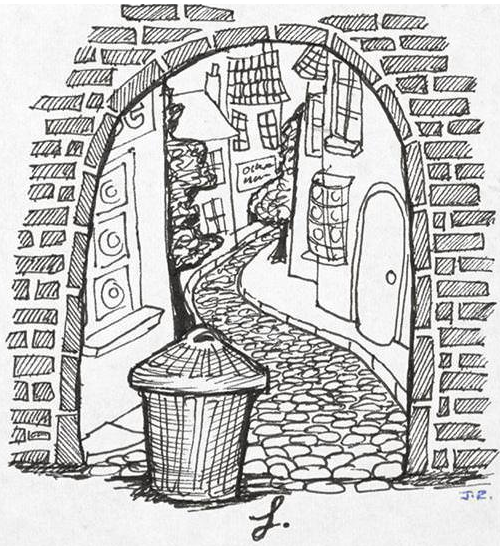
\includegraphics[scale = 0.6]{../../Images/alley} % also works with logo.pdf
    \vfill
    {\HP \fontsize{30}{24} \selectfont  Harry Potter \\\&\\ The Role Playing Game}
    \normalsize
    \vfill
    {\HP \fontsize{22}{0} \selectfont Version 1.0 \hfill Jack Fraser}
\end{titlepage}



	\renewcommand\arraystretch{1.5}
\newcommand\basicPerson[2]
{
	\textbf{\textit{#1}}
	
	#2

}

\newcommand\invent[3]
{
	\hline	 \parbox[t]{3cm}{\raggedright #1}	&	\it #2	&	#3  \\
}

\newcommand\inventLine[3]
{
	{\bf #1} (#3) {\it #2} \\
}

\newcommand\expand[2]
{
	\subsection{Expanded Inventory For #1}
	~
	\tablealternate
	\begin{supertabular}{@{} |p{3cm} |p{4cm} |m{0.5cm}|}
	\hline
	\tableheader \bf Name	&	\bf Description 	&	\bf Cost \\ \hline
		#2 \hline
	\end{supertabular}
	\vfill
	

}

\newcommand\shop[7]
{
	\subsection{#1 (\it #4)}
	
	\begin{supertabular}{@{} r p{6.5  cm} @{}}
		\bf Location:	&	#2
		\\
		\bf Exterior: &		#5
		\\
		\bf Interior:	&	#6
		\\
		\bf Proprietor:	&	#3
		\\
		
		
	\end{supertabular}
	
	{\bf Inventory:}	~	\parbox[t]{6.5cm}{#7}
	\\
}

\setlength\parindent{3pt}
%%ShopBegin
\shop{Eeylops Owl Emporium}{Diagon Alley}{\basicPerson{Frank Blumenthal}{A dour faced man\comma{} who seems not to care for humans whatsoever. Where possible\comma{} he uses a single word to answer a question\comma{} before returning to his owls. 

He only ever cracks a smile when talking about his birds\comma{} which are his whole world. He will refuse to sell an owl if he believes it will be maltreated.} }{Owls}{A huge number of vertical poles stand outside this shop. During daytime\comma{} a multitude of different colour owls occupy them\comma{} cooing and hooting to one another.}{Inside\comma{} the ceiling reaches all the way to the rafters\comma{} creating a very tall (if narrow) space for the owls to fly. Birdcages line the wall\comma{} though the owls themselves seem to roost in special nooks in the walls above headheight.}{A pet owl costs \galleon{1}\comma{} though some of the finer species cost significantly more.}

\shop{Florean Fortescue\apos{}s Ice Cream Parlour}{Diagon Alley}{\basicPerson{Sylvian Fortescue}{The twin brother of the eponymous original proprietor\comma{} Sylvian is an elderly man in his late 90s: balding and with a hooked nose. 

Though elderly in appearance\comma{} he harbours a twinkle in his eye and a spring in his step. A Wonka\minus{}esque pioneer of flavours\comma{} he seems much younger than his advanced years.} }{Ice cream parlour}{A handful of chairs and small tables\comma{} with sunshades\comma{} all a light duck\minus{}egg blue sit outside the storefront\comma{} which (on sunny days) is fully opened to expose the interior to the outside world.}{More chairs and tables are inside the brightly lit interior\comma{} along with a front desk harbouring thousand of flavours of icecream � a multicoloured medly of flavour and sweetness.}{Icecream costs \knut{5} a scoop. 

If you can imagine a flavour\comma{} they have it\comma{} no matter how odd.}

\shop{Flourish \& Blotts}{Diagon Alley}{\basicPerson{Sam Garret}{A severe looking woman with small glasses � your stereotypical high school librarian. 

Though fierce looking\comma{} she takes delight in helping people find the books they need.} }{Books}{A well kept storefront\comma{} with a clean window that allows one to see the bookshelves inside. 

A number of placards out front advertise new arrivals and special offers.}{A central desk is surrounded by hundreds\comma{} thousands of books\comma{} stuffed into bookshelves which line every wall. There us a set of stairs up to another level (with yet more books)\comma{} and several small stepladders float up to customers to help them reach high shelves.}{A full inventory for this shop can be found at the end  of the document}

\shop{Gringotts Bank}{Diagon Alley}{\basicPerson{Grp\apos{}tar}{An aging goblin\comma{} who serves as the primary point of contact for new arrivals\comma{} before directing them to a teller or into the vaults. 

His eyes hold suspicion for everyone\comma{} and he has a distrustful\comma{} dismissive air.} }{Bank}{An enourmous marble clad bulding. A set of marble steps lead visitors up into a giant pillared rotunda with a sky\minus{}blue roof.}{The vast entryway opens up into a large hall\comma{} lined with goblin tellers stacking and counting piles of gold and jewels\comma{} or seeing to customers. 

The proprietor sits on a raised dias in the centre of the hallway. Behind him in a secured area is the entrance to the lower vaults.}{N/A}

\shop{Leaky Cauldron}{Diagon Alley}{\basicPerson{Hannah Abbot}{A blonde lady in her early forties\comma{} with a smiling face and kind eyes. 

Though mostly an unassuming landlady\comma{} under the surface is a trained battlemage � as a member of the DA she faced Voldemort and his Death Eaters. She is currently married to Neville Longbottom.} }{Pub \& Inn}{An old fashioned inn\comma{} above the dorr is mounted a hanging caldron\comma{} perpetually pouring a purple fluid out of it.}{Surprisingly modern\comma{} the wood\minus{}panelled bar area is clean and the smell of cooking food pervades. 

There are several private parlours behind the bar area.}{Soup of the day (\knut{10} )

Hearty Meal (\sickle{4} ) 

Butterbeer (\sickle{2} )

Fire Whiskey (\sickle{2} )}

\shop{Madam Malkin\apos{}s Robes for All Occasions}{Diagon Alley}{\basicPerson{Madam Malkin}{An effortlessly beautiful half\minus{}veela\comma{} everything she does is suffused with elegance and grace. 

She treats every customer as if they were the centre of her entire world\comma{} her warm words layered with kindness and compliments.} }{Clothing}{A simple\comma{} yet stylish storefront. The wooden panelling is freshly painted black\comma{} and shines in sunlight. 

The display window showcases three mannequins in the finest outfits for witches and wizards. 

The sign above the door simply reads {\it MM} in a fancy font.}{Clothing racks towards the front of the store hold numerous robes and outfits of different types. 

Towards the back of the store is an open area where customers go to get measured for custom orders.}{A full inventory for this shop can be found at the end  of the document}

\shop{Magical Menagerie}{Diagon Alley}{\basicPerson{Tom Cove}{A short\comma{} squat and unusually ugly man\comma{} with a mess of black hair and lopsided and mishapen features. 

What he lacks in good looks\comma{} he makes up for in charm and personality. A natural salesman and a people person\comma{} he drives a hard bargain.} }{Pets}{The front window of the shop has been converted into a display containing a Murtlap burrow\comma{} such that you can see the underground structure pressed between the glass plates}{The interior contains rows upon rows of cages and tanks of various sizes\comma{} some containing entire ecosystems inside them.}{A full inventory for this shop can be found at the end  of the document}

\shop{Ollivander\apos{}s}{Diagon Alley}{\basicPerson{Jenna Ollivander}{A young woman in her early thirties\comma{} though with a shock of grey\minus{}white hair which sticks out at odd angles. 

She is excitable\comma{} and has a nervous energy as she darts around her shop\comma{} jumping and skipping as she goes. Though the boxes have no labels\comma{} she seems to be able to find whatever she is looking for.} }{Magical wands}{A tall\comma{} narrow building barely wide enough to fit two people abrest. 

The green sign above the door has the name written in large golden letters.}{Narrow and cramped\comma{} with every wall covered in row upon row of wandboxes. The light is suffused with  magical energy.}{Ollivander\apos{}s has all normal wands for sale at \galleon{5} each. To buy a wand\comma{} you must roll on the wand table.}

\shop{Quality Quidditch Supplies}{Diagon Alley}{\basicPerson{Seamus Finnigan}{An irish gentleman\comma{} in his mid\minus{}forties and the lack of hair to prove it. 

Deeply passionate about quidditch\comma{} he will talk for hours to customers about their purchases\comma{} and ensure they have exactly what they need.} }{Brooms}{A large window display prominently shows the latest model of broomstick\comma{} as well as mannequins wearing the uniforms for some of the larger quidditch teams.}{Wall\minus{}mounted racks hold many different broomsticks\comma{} and a number of snitches buzz around in the air buffeting into customers.}{\inventLine{Cleansweep 10~($\times$5)}{The latest in the cleansweep range. Not a flashy broomstick\comma{} but enough to get you around.}{\galleon{40}}
\inventLine{Comet 530~($\times$10)}{The Comet has never been a flashy brand. This is their latest low\minus{}cost broomstick. It handles like a cow\comma{} but for the price\comma{} it really is quite good.}{\galleon{50}}
\inventLine{Thunderbolt~($\times$2)}{A newcomer to the scene \minus{} the Thunderbolt has cast off much of what we know about broomsticks\comma{} and reinvented many basic principles. An aluminium frame is just the start. Is this the future of flight? We don\apos{}t know\comma{} but it could be!}{\galleon{300}}
\inventLine{Firebolt X~($\times$1)}{A few years behind the latest brands now\comma{} but nothing beats the Firebolt in terms of raw speed and\comma{} oh boy\comma{} does it look good.}{\galleon{500}}
\inventLine{Nimbus 2020~($\times$1)}{The newest\comma{} shiniest broomstick around. The Nimbus 2020 boasts enourmous speeds\comma{} and the revolutionary inertial dampners\comma{} which allows you to take accelerations which would kill a normal wizard.}{\galleon{700}}
}

\shop{Rosa Lee Teashop}{Diagon Alley}{\basicPerson{Rosa Lee}{A short\comma{} plump lady dressed all in purple � including dyed purple hair. 

Homely and kind\comma{} she takes joy in feeding people\comma{} and will often slip an extra slice onto the plates of those she thinks are a bit malnourished.} }{Food \& Drink}{A quaint little teashop\comma{} with a purple exterior. A large window opens onto the kitchen\minus{}area\comma{} showing a set of enchanted kitchen tools preparing fresh cakes.}{Inside is an explosion of colour: paisly tablecloths and tartan teapots\comma{} with polka dot chairs. 

Nothing matches\comma{} and everything is garish � and yet it somehow manages to avoid crossing the line into tacky.}{Afternoon tea (\sickle{5})

Slice of cake (\knut{15} )}

\shop{Slug \& Jiggers Apothecary}{Diagon Alley}{\basicPerson{Jemima Poffley}{A young woman in her mid\minus{}twenties\comma{} with closely cropped hair and a large pair of glasses. 

She has a nervous stutter\comma{} and seem unsure of herself � until she starts talking about alchemy and potions.} }{Potions}{The outside of the shop is almost entiely obscured by a thick rolling fog that seems to be coming from a top floor window. Every few minutes\comma{} there�s a loud {\it crack} sound\comma{} and the colour of the smoke changes � usually accompanied by some choice curses.}{Inside the air is clean and fresh\comma{} and smells of fresh picked grass and other herbs. 

Rows upon rows of jars line the walls\comma{} all meticulously labelled. 

The centre of the room has some larger merchandise � cauldrons and alchemical filters.}{There are 5 samples of each potion available.A full inventory for this shop can be found at the end  of the document}

\shop{Sugarplum Sweetshop}{Diagon Alley}{\basicPerson{Jo King}{An elderly man\comma{} with bright blue hair\comma{} and only a single tooth. 

A talks with a lisp\comma{} but is full of vim and vigour. He has a special (non creepy) fondness for children\comma{} and delights in finding them new sweets that they have  never experienced before.} }{Sweets}{The window is stacked full of displays showcasing sweets and treats � from old favourites to the newest imports. 

A goblin employee outside stands with a tray of free samples\comma{} attempting (though mostly failing) to entice people inside.}{An amazingly stocked\comma{} traditional sweet shop. Enormous jars filled with goodies line every wall\comma{} and children dart around filling up paper bags with their favourite sweets.}{Acid Pops (\knut{12})

Bertie Botts Every Flavour Beans (\knut{5})

Chocolate Frogs (pack of 3 \minus{} \sickle{1})

Fizzing Whisbees (\sickle{1})

Liquorice Wands (\knut{15})}

\shop{The Junk Shop}{Diagon Alley}{\basicPerson{Lomp}{Unmistakeably a man with significant amounts of giant blood in him\comma{} Lomp stands a full 7 feet tall\comma{} and seems almost as wide. 

Matted blond hair falls to his mid back\comma{} and his outfit is an insane medley of colours and styles. His fingers have an assortment of rings and other decorations (most of which are hideous and obviously made of actual rubbish). 

He is very possessive of the stuff in his shop\comma{} and gets very defensive when it is insulted as useless.} }{Various}{The exterior of this shop is almost non\minus{}existent � it is simply a door wedged inside a great mound of crates stacked outside the font of the shop\comma{} obscuring everything else about the bulding and spilling out onto the street.}{A dark\comma{} fusty and cramped interior\comma{} the room is filled with rows upon rows of shelves covered in what is almost entirely rubbish. 

The stuff does not smell\comma{} but it comprises of broken pottery and dented metal plates\comma{}  Threadbare blankets and two\minus{}legged chairs.}{Most of the stuff in this shop is pure junk. Though on a successful DV12 Investigation check\comma{} a number of worthwhile items can be found. 

~A full inventory for this shop can be found at the end  of the document}

\shop{The Newt\apos{}s Eye}{Diagon Alley}{\basicPerson{Jean\minus{}Luc Appelard}{The most stereotypical frenchman you will ever meet. He speaks with a flourish\comma{} and carries a baguette under one arm. He looks with disdain on the silly englishmen\comma{} though he is more than happy to take their money. 

The rumour is that his true name is Frank Butterworth\comma{} and that he accidentally consumed a herb which caused him to act this way.} }{Alchemical Supplies}{This store is abviously well\minus{}looked after\comma{} and is meticulously clean. 

A number of racks of herbs and other alchemical supplies stand out the front to dry and for display purposes.}{Inside the same meticulous air is apparent\comma{} with every alchemical supply neatly stored inside a perfectly clean jar. The jars themselves are all perfectly aligned and have labels written in exactly the same neat hand.}{A full inventory for this shop can be found at the end  of the document}

\shop{Weasley\apos{}s Wizard Wheezes}{Diagon Alley}{\basicPerson{George Weasley}{A one\minus{}eared\comma{} red\minus{}haired jokester\comma{} who spends most of his time playing pranks on his customers\comma{} rather than trying to sell them anything. 

Unusually\comma{} however\comma{} this business model has turned out to be an incredible success\comma{} and George and his brother Ron have turned this into a successful business.} }{Prank shop}{A prominent shop\comma{} right on the street corner\comma{} made even more noticeable by the large weasley\minus{}esque statue mounted atop the frontage. This statue is known to make rude gestures and blow raspberries at passers by.}{A wide open shop floor\comma{} with a cacophany of noise as George prances round\comma{} demonstrating his wares. 

Small alcoves are found at the back where the pricier items are held\comma{} and in the front are vast vats of their best selling items.}{A full inventory for this shop can be found at the end  of the document}

\shop{Wiseacre\apos{}s Wizarding Equipment}{Diagon Alley}{\basicPerson{Ralph Wisacre}{The ghost of a man in his mid 50s\comma{} whispy hair (difficult to tell what colour it was\comma{} given he is dead)\comma{} who has been running this store (with a little corporeal help) for nearly 1000 years. 

He specialises in magically enchanted items\comma{} and has a gift for spotting the worth of items.} }{Enchanted Items}{A modest building\comma{} the window display shows several enchanted items: a flying rug hovers above a pedestal displaying a glowing genie\apos{}s lantern\comma{} whilst a cloak glows with runes off to one side.}{Inside is barely lit\comma{} except for a little torchlight which casts odd shadows. The merchandise is stored in low glass cabinets. 

You get the sense that this is all entirely for show\comma{} to bring an air of mystique to the business.}{A full inventory for this shop can be found at the end  of the document}

\shop{Borgin \& Burke\apos{}s}{Nockturn Alley}{\basicPerson{Mr Borgin}{An oily\comma{} creepy gentleman\comma{} Mr Borgin is wholly unpleasant. He is obsessed with money\comma{} and seems not to care if he earns it by selling dangerous and evil artefacts. 

He will buy and sell anything: stolen\comma{} cursed or downright posessed by demonic forces; as long as there is profit involved.} }{Dark Magic}{The front of the shop is painted in green paint\comma{} which is in need of dire repair as it cracks and falls off. 

The windows are grubby and oily\comma{} and have a weird sheen to them that you cannot quite indentify.}{Inside\comma{} cobwebs and dust abound\comma{} giving an air that this shop has long been abandoned\comma{} despite the evidence to the contrary. 

Items lies on gilded pillow cases and in tall display cases\comma{} meticulously labelled in spindly handwriting.}{A full inventory for this shop can be found at the end  of the document}

\shop{Cobb and Webb\apos{}s}{Nockturn Alley}{\basicPerson{Spinstress Simone Belvoire}{Just by looking at this elderly lady\comma{} you can tell she has an unhealthy obsession with arachnids. 

Her hair is pinned back with a spider hair pin\comma{} and spider badges and jewellery adorn her person. 

She speaks in a soft\comma{} slow voice. She is kind\comma{} but very creepy.} }{Spiders \& Necromancy}{The most prominent feature of the shopfront is an enormous gothic stained glass window showing a black widow spider devouring her prey.}{Inside the spider theme continues\comma{} with live specimens crawling all over the walls. Almost all the merchandise is spider\minus{}related\comma{} though there are a few generic Dark Arts books.}{\inventLine{Necromancy: A Misunderstood Skill~($\times$3)}{A book of beginner level Necromancy magic}{\galleon{2}}
\inventLine{An A\minus{}Z of Spooky Spells~($\times$3)}{A book of beginner level Occultism magic}{\sickle{16}}
\inventLine{The Forbidden Arts~($\times$2)}{A book of novice level Necromancy magic}{\galleon{6}}
\inventLine{Rehabilitating Blood and Darkness in Everyday Magic~($\times$2)}{A book of novice level Occultism magic}{\galleon{2}}
\inventLine{Living in Shadow: The Memoirs of an Occultist~($\times$1)}{A book of adept level Occultism magic}{\galleon{4}}
}

\shop{Hagg\apos{}s Feast}{Nockturn Alley}{\basicPerson{Rinna the Mad}{You can\apos{}t quite decide if Rinna is an elderly and slightly insane which\comma{} or an actual Hag. 

Certainly\comma{} her mannerisms\comma{} pointed teeth and warted face point to the latter\comma{} and she has an unsettling habit of cackling maniacally.} }{Meat}{The shop window has been totally blacked out\comma{} as if the proprietor doesn't like sunlight.}{Inside there are display units showing all kinds of exotic meats. You\apos{}re somewhat afraid to ask what some of the meat is\comma{} especially the stuff that still seems to be moving.}{If you can kill it and eat it\comma{} you can buy it here. Prices start at \sickle{10}\comma{} and go up from there.}

\shop{Mulpepper\apos{}s Apothecary}{Nockturn Alley}{\basicPerson{Mary Mulpepper III}{A sweet and charming lady in her 30s. She has dark brown hair and cheerful eyes. 

Despite her outwardly beautiful appearance\comma{} it is disturbing to hear her talk so openly and candildly about the viciousness of some of the alchemical ingredients she harbours and the potential uses for them.} }{Dangerous Alchemical Ingredients}{The window is blotted out by stacks and stacks of grubby jars\comma{} filled with a green fluid\comma{} in which float shadows which suggest horrifying contents.}{Inside there are yet more jars\comma{} with their floating contents slowly picklilng away. 

There are also some dry goods to be found in the centre of the shop.}{A full inventory for this shop can be found at the end  of the document}

\shop{Shyverwretch\apos{}s Venoms and Poisons}{Nockturn Alley}{\basicPerson{Wendy}{Wendy is a (former) House\minus{}Elf\comma{} and now a member of the Free Elf establishment. 

Her former master was the owner of this establishment\comma{} until he met a sticky end\comma{} and if the rumours are to be believed\comma{} his servant had something to do with it.  

Wendy seems like a cheerful house elf\comma{} but occasionally the mask slips and reveals a deep sociopathic streak beneath the surface.} }{Poisons}{Delicate glass vials are stacked neatly in the window. They would be beautiiful\comma{} were it not for the ugly colouration of some of them.}{Inside there are more glass jars\comma{} and more suspect liquids. 

Your nose burns with the acrid atmosphere\comma{} though Wendy doesn\apos{}t seem to notice.}{A full inventory for this shop can be found at the end  of the document}

\shop{The Coffin House}{Nockturn Alley}{\basicPerson{N/A}{N/A} }{Dangerous Black Magic}{The smashed in front door and the official\minus{}looking Auror tape outside indicate that this shop was recently raided and shut down by the ministry\comma{} presumably for conducting some heinous black\minus{}magic crime.}{The inside is charred and still lightly smoking. It looks like a large magical battle was fought here\comma{} and a slight metallic smell in the air hint at a large amount of bloodshed.}{N/A}

\shop{White Wyvern}{Nockturn Alley}{\basicPerson{Gnarlock}{A young but visibly battle\minus{}scarred goblin. Gnarlock has no time for humans unless they\apos{}re putting coin into his pocket. 

Dismissive and gruff\comma{} he is unpleasant to everyone and anyone\comma{} but {\it especially} newcomers.} }{Pub \& Inn}{A dilapidated old pub\comma{} with a rusted sign depicting a dragon. From the name\comma{} you presume it used to be white\comma{} but the sign is more of a grubby grey nowadays.}{Inside is dark and dank. Hooded patrons sit at the bar muttering to one another. 

When newcomers arrive\comma{} they all turn to look at them with suspicion in their eyes.}{Fire whiskey (\knut{10})}

\shop{Daily Prophet HQ}{Venter Alley}{\basicPerson{Barnabus Cuffe}{The editor\minus{}in\minus{}chief of the Daily Prophet for several decades\comma{} Barnabus Cuffe is an affable gentleman � always seen wearing an impeccable suit and tie underneath a formal wizarding gown. 

His affable demeanor is\comma{} however\comma{} mostly for show and beneath the surface he is a man consumed with the need to accumulate and gather power and influence. He will let nothing (let alone the truth) get in the way of his media empire.} }{Newspaper Printers}{An unassuming building\comma{} without a formal shopfront. 

The only indicators that this is anything other than a residential house is a formal plaque next to the door\comma{} and a dispenser for the Daily Prophet on the street outside.}{The interior is significantly larger than the exterior\comma{} and houses a full magical printing press\comma{} as well as several offices for the prominent journalists. 

The office of the editor is on the second level\comma{} but with a large window capable of overseeing the entire operation.}{Daily Prophet (\knut{8})}

\shop{Flibberdigibits \& Watchemacallems}{Venter Alley}{\basicPerson{Store Clerk}{A fairly faceless employee of this chain of grocery stores. He has a slightly vacant expression as he processes your order\comma{} but he seems nice.} }{Groceries}{This shop looks almost identical to all the others in the chain \minus{} a bright blue storefront\comma{} with signs and placards indicating the current deals.}{Inside there are rows and rows of fresh produce from around the world\comma{} including some muggle goods that have caught on lately.}{Roughly \sickle{3} for enough food to feed one person for one day.}

\shop{Ministry of Magic}{Venter Alley}{\basicPerson{Galen Rex}{The new Minister for Magic\comma{} who rode into power on a populist wave\comma{} after widespread unease at the liberalising reforms made by the previous minister. 

Galen is a former Healer by trade\comma{} turned to politics. He is charming and suave\comma{} though his political views and methods have caused many to question his ethics\comma{} he is incredibly popular.} }{Government}{The Ministry is mostly operated underground (underneath what the muggles refer to as Leicester Square)\comma{} however there is a majestic open\minus{}air entrance at the end of Venter Alley.

A wide open plaza full of statues of famous witches and wizards throughout the ages can be found. The square is normally full of bustling tourists and ministry workers alike.}{The atrium of the ministry is covered with midnight\minus{}blue tiles in a forum that (even though from outside it seemed only two or three stories tall) stretches up into immense heights. Enchanted messages flit from side to side\comma{} and there is a continual foot traffic as employees rush through this nexus.}{N/A}

\shop{Simon\apos{}s Simple Shields}{Venter Alley}{\basicPerson{Simple Simon}{Don\apos{}t let his name fool you \minus{} this blonde\minus{}haired blued eyes supermodel is incredibly intelligent. 

He prefers to cultivate an air which lets others underestimate him\comma{} and so he often mans his store topless and with a gormless stare. When it comes down actual business\comma{} however\comma{} you find him a ruthless negotiator.} }{Defensive Armour}{Above the door\comma{} two strong iron shields are set. 

If you enter with ill\minus{}intent\comma{} the shields ignite with a fiery glow\comma{} and a forcefield expels you out of the front door.}{Inside is incredibly hot\comma{} as Simon attends to the forge which he magically shields to keep the worst of the heat out. 

Shields and armour both magical and mundane are lying around in a clutter. There seems to be no rhyme or reason as to the placement of the objects in this shop.}{A full inventory for this shop can be found at the end  of the document}

\shop{Warcasters}{Venter Alley}{\basicPerson{Longtail}{An incredibly unusual sight outside of their forested domains: Longtail is a centaur. 

Even more unusually\comma{} he is not involved in the usual divination magic. Longtail was a Sentinel for his clan\comma{} before being kicked out for his extremist views regarding the merpeople. 

Now he uses his martial prowess to make a profit by smithing and creating weapons\comma{} both magical and mundane.} }{Offensive Weapons}{In the shop window is a single stand\comma{} holding a magnificent glowing greatsword. 

Through the sword itself seems perfectly ordinary\comma{} there is a magical aura that causes passers by to stop and gape at it.}{Inside more weapons can be found\comma{} strapped meticulously in order\comma{} arranged by type\comma{} price and enchantment level. 

The air is heavy with the scent of weapon oil and magic.}{A full inventory for this shop can be found at the end  of the document}

\section{Expanded Inventory} \footnotesize 


\expand{Flourish \& Blotts}{\invent{Lighting the Spark: An Introduction to Elemental Magic~($\times$3)}{Book of Beginner Elemental spells}{\sickle{10}}
\invent{The Standard Book of Spells~($\times$3)}{Book of Beginner Kinesis spells}{\sickle{10}}
\invent{Reading People\comma{} Reading Minds~($\times$3)}{Book of Beginner Telepathy spells}{\sickle{10}}
\invent{The Dream Oracle~($\times$3)}{Book of Beginner Temporal spells}{\sickle{10}}
\invent{Easy Spells to Fool Muggles~($\times$3)}{Book of Beginner Bewitchment spells}{\sickle{10}}
\invent{Cool Cantrips to Make You Crazy~($\times$3)}{Book of Beginner Psionics spells}{\sickle{10}}
\invent{A Compendium of Common Curses~($\times$3)}{Book of Beginner Curse spells}{\sickle{10}}
\invent{Basic Hexes for the Busy \& Vexed~($\times$3)}{Book of Beginner Hex spells}{\sickle{10}}
\invent{Cures\comma{} Cantrips and Coughs~($\times$3)}{Book of Beginner Healing spells}{\sickle{10}}
\invent{Self\minus{}Defensive Spellwork~($\times$3)}{Book of Beginner Warding spells}{\sickle{10}}
\invent{A Beginner\apos{}s Guide to Transfiguration~($\times$3)}{Book of Beginner Alteration spells}{\sickle{10}}
\invent{The Illusion of {\it Thin Air}~($\times$3)}{Book of Beginner Conjuration spells}{\sickle{10}}
\invent{Further Elemental Studies~($\times$2)}{Book of Novice Elemental spells}{\galleon{1}}
\invent{Achievements in Charming~($\times$2)}{Book of Novice Kinesis spells}{\galleon{1}}
\invent{Detection is the Best Defense~($\times$2)}{Book of Novice Telepathy spells}{\galleon{1}}
\invent{The Future is an Open Book (And so is This)~($\times$2)}{Book of Novice Temporal spells}{\galleon{1}}
\invent{Jiggery Pockery \& Hocus Pocus~($\times$2)}{Book of Novice Bewitchment spells}{\galleon{1}}
\invent{Your Mind\comma{} the Weapon~($\times$2)}{Book of Novice Psionics spells}{\galleon{1}}
\invent{Curses \& Counter Curses~($\times$2)}{Book of Novice Curse spells}{\galleon{1}}
\invent{Hexes to Make Your Head Spin (Literally)~($\times$2)}{Book of Novice Hex spells}{\galleon{1}}
\invent{Magic to Make Others Better~($\times$2)}{Book of Novice Healing spells}{\galleon{1}}
\invent{How Not to be Killed: A Guide for the Discerning Wizard~($\times$2)}{Book of Novice Warding spells}{\galleon{1}}
\invent{Transmutation and Transformative Tricks~($\times$2)}{Book of Novice Alteration spells}{\galleon{1}}
\invent{Making and Unmaking: The Art of Conjuration~($\times$2)}{Book of Novice Conjuration spells}{\galleon{1}}
\invent{Runic Scroll~($\times$4)}{Provides 1 additional rune}{\sickle{8}}
\invent{Small Maps~($\times$5)}{Provides information about a single village or town}{\sickle{5}}
\invent{Large Maps~($\times$5)}{Maps of large cities\comma{} and even entire countries.}{\sickle{8}}
\invent{Fantastic Beasts and Where to Find Them~($\times$3)}{Provides basic information about common beasts}{\sickle{12}}
\invent{The Unlife \& How to Avoid Them~($\times$1)}{Provides basic information about undead \& unliving creatures}{\galleon{1}}
\invent{Monster Book of Monsters~($\times$2)}{A sentient book which viciously attacks people \minus{} inside it has detailed information about common beasts.}{\galleon{1}}
\invent{Rare and Dangerous Magical Creatures Aruond the World~($\times$1)}{Provides basic information about some of the rarer magical creatures found in the world.}{\galleon{2}}
\invent{One Thousand Magical Herbs \& Fungi~($\times$5)}{Contains information about ingredients \& gives hints as to potions they can be used in.}{\sickle{10}}
\invent{Wizarding Biographies~($\times$5)}{Biographies of some famous wizards}{\sickle{7}}
\invent{Potion books~($\times$5)}{Each contains 1d8 random recipes for potions}{\sickle{10}}
}

\expand{Madam Malkin\apos{}s Robes for All Occasions}{\invent{Ball Gown~($\times$5)}{A beautifulrack of ball gowns in a variety of styles \minus{} some backless \& sheer\comma{} others poofy and voluminous. Perfect {\it Formal Wear}.}{\galleon{2}}
\invent{Chameleon Robes~($\times$1)}{A set of robes interwoven with the hair of several colour\minus{}changing species. Not a perfect invisibility cloak\comma{} but the shifting patterns make one much harder to see whislt wearing it.}{\galleon{10}}
\invent{Dragonhide Gloves~($\times$2)}{Beautiful {\it and} practical! These iridescent green gloves shield your hands entirely from the effects of both great heat\comma{} and great cold.}{\galleon{3}\sickle{11}}
\invent{Dress Robes~($\times$5)}{An exquisitely ornamental set of wizards robes in a variety of colours\comma{} with frills\comma{} ruffs and all the trimmings. Potentially a little dated on someone below the age of 50\comma{} but still vaguely fashionable . Perfect {\it Formal Wear}}{\galleon{2}}
\invent{Hogwarts Uniform~($\times$25)}{A set of finely made {\it Wizards Robes}\comma{} embroided with one of the four house crests of Hogwarts.}{\sickle{10}}
\invent{Self Repairing Jacket~($\times$4)}{An extension on Malkin\apos{}s informal range \minus{} this upmarket jacket repairs itself after taking damage.}{\galleon{4}}
\invent{Stylish Leather Jacket~($\times$5)}{A stylish leather jacket \minus{} part of Malkin\apos{}s new informal range.}{\sickle{14}}
\invent{Tuxedo~($\times$5)}{A finely made tuxedo set\comma{} complete with a bow tie. Perfect {\it Formal Wear}}{\galleon{1} \sickle{10}}
\invent{Custom Made~($\times$3)}{Madame Malkin is happy to take custom orders for her work \minus{} as long as it is within her skillset.}{\galleon{5}}
}

\expand{Magical Menagerie}{\invent{Cat~($\times$10)}{Numerous different breeds of cats \minus{} from tabbies\comma{} to black cats and long haired ginger beasts.}{\sickle{8}}
\invent{Crow~($\times$5)}{A slightly dumber raven. Their feathers are less sleek\comma{} and their beaks less razor sharp \minus{} perfect for the first\minus{}time bird keeper.}{\sickle{6}}
\invent{Flobberworm~($\times$100)}{Ugh. Giant\comma{} slobbering worms. They haveno brain to speak of\comma{} and their actions betray that.}{\knut{10}}
\invent{Kneazle~($\times$4)}{A full\minus{}blooded kneazle\comma{} capable of seeing into the future and protecting you from harm. Very rare.}{\galleon{15}}
\invent{Kneazle\minus{}Cat~($\times$8)}{A highly\minus{}intelligent species of cat\comma{} with some kneazle blood. They alert their owners when danger is near.}{\galleon{3}}
\invent{Nifflers~($\times$10)}{A small brood of baby nifflers\comma{} they imprint on their first owner like a mother. Incredibly cute \minus{} but watch your jewellery!}{\sickle{10}}
\invent{Puffskein~($\times$20)}{A fat little ball of pink fluff\comma{} with an enourmously long tongue that drifts out of it. Very cute and cuddly.}{\sickle{10}}
\invent{Rabbit~($\times$5)}{Floppy eared\comma{} and noses a\minus{}wrinkling. Very cute as pets\comma{} or for pulling out of a hat.}{\sickle{6}}
\invent{Rat~($\times$5)}{It's a rat. Clean and friendly\comma{} but a rat.}{\sickle{3}}
\invent{Raven~($\times$1)}{An unusual substitute for the usual owl\comma{} usually reserved for the more�goth�wizards. A crow is however\comma{} incredibly intelligent\comma{} and can be trained to mimic human speech.}{\galleon{1}}
\invent{Snowy Owl~($\times$3)}{A beautiful white oel. Trained to deliver post.}{\sickle{15}}
\invent{Tarantula~($\times$3)}{Creepy crawly\comma{} but some claim also mesmerising. This black\comma{} hairy specimen has highlights of bright orange.}{\sickle{10}}
\invent{Tawny Owl~($\times$6)}{A mottled brown owl. Trained to deliver post.}{\sickle{10}}
\invent{Toad~($\times$4)}{A fat\comma{} squat animal. They might seem like terrible pets\comma{} but they are surprisingly affectionate and very hard to kill.}{\sickle{15}}
}

\expand{Slug \& Jiggers Apothecary}{\invent{Alchemy Gear~($\times$2)}{A set of high\minus{}quality alchemy gear\comma{} needed for mixing potions.}{\sickle{15}}
\invent{Herbology Tools~($\times$5)}{Tools needed to extract delicate samples from beings and plants.}{\sickle{9}}
\invent{Alihotsy Draught~($\times$4)}{Causes uncontrollable fits of laughter\comma{} preventing the target from speaking for 2 minutes}{\sickle{9}}
\invent{Antidote to Common Poisons~($\times$4)}{Reduce the remaining time left on an ongoing potion effect by 25 \%}{\sickle{7}}
\invent{Anti\minus{}Paralysis Potion~($\times$4)}{Rejuvinate the drinker. Removes the {\it Paralyzed} status and restores FP by 4 points}{\sickle{9}}
\invent{Azimov\apos{}s Awesome Acid~($\times$4)}{Do not drink! Destroys armour\comma{} reducing {\it Block} statistic by 2 points}{\sickle{11}}
\invent{Baruffio\apos{}s Brain Elixir~($\times$4)}{For one hour\comma{} gain an intelligence boost of 2 points}{\galleon{2}}
\invent{Blemish Blitzer~($\times$4)}{When applied to the skin\comma{} instantly removes all rashes\comma{} acne\comma{} boils and other skin ailments and restores HP by 2 points}{\sickle{7}}
\invent{Blood\minus{}Refilling Potion~($\times$4)}{For 5 minutes after being drunk\comma{} causes HP to regenerate at a rate of 2 per round}{\galleon{3} \sickle{10}}
\invent{Burn\minus{}healing paste~($\times$4)}{When applied to the skin\comma{} removes the {\it Burned: Mild} status effect and leaves the target Resistant to Fire damage for 2 minutes}{\sickle{9}}
\invent{Calming Draught~($\times$4)}{Calms and soothes the target\comma{} and makes them immune to the {\it Terrified} status and {\it Rage} effect for 2 minutes}{\sickle{9}}
\invent{Curse\minus{}Countering Concoction~($\times$4)}{Target is immune to spells from the {\it Curse} discipline for 2 minutes}{\galleon{10} \sickle{15}}
\invent{Draconic Protection Draught~($\times$4)}{The drinker\apos{}s skin develops scales\comma{} increasing {\it Block} statistic by 2 points}{\sickle{11}}
\invent{Dragonbreath Solution~($\times$4)}{Gain the ability to summon a gout of fire from your mouth in a cone 2m long\comma{} doing 3d8 fire damage for 30 seconds}{\galleon{3} \sickle{10}}
\invent{Drink of Despair~($\times$4)}{When consumed\comma{} the victim becomes {\it Terrified} of a random object within sight for 5 minutes}{\galleon{2}}
\invent{Emanation Elimination Elixir~($\times$4)}{This potion is not drunk\comma{} but released into the atmosphere. It repels all gases\comma{} odours and other atmospheric effects in a radius of 5 metres}{\sickle{13}}
\invent{Fatiguing Infusion~($\times$4)}{Drains the afflicted of 10 FP}{\galleon{1} \sickle{5}}
\invent{Final Goodnight~($\times$4)}{Applies the {\it Poisoned: Severe} status effect and immediately deals 50 Poison Damage}{\galleon{65} \sickle{5}}
\invent{Flask of Freezing~($\times$4)}{When the cork is removed from the phial\comma{} the liquid expands into an arctic vortex\comma{} freezing water and dealing 5d4 cold damage in a radius of 4 Metres}{\galleon{10} \sickle{15}}
\invent{Growing Agent~($\times$4)}{When applied to a living being\comma{} causes it to grow in size by 50 \%}{\galleon{1} \sickle{5}}
\invent{Herbicide Potion~($\times$4)}{When dropped on the ground\comma{} kills all plants in a radius of 5 metres}{\sickle{9}}
\invent{Hero\apos{}s Brew~($\times$4)}{The cowardly consumer of this potion finds themselves immune to the {\it Terrified} status effect. 10 minutes}{\sickle{9}}
\invent{Infusion of Strength~($\times$4)}{For one hour\comma{} the drinker gets a bonus to checks that use the Strength proficiency by 2 points}{\galleon{3} \sickle{10}}
\invent{Insulation Inocculation~($\times$4)}{When consumed\comma{} cures a target of the {\it Frostbite: Mild} status\comma{} and prevents it from being reacquired for 10 minutes}{\sickle{15}}
\invent{Mopsus\apos{} Tincture~($\times$4)}{Opens your inner eye for 5 minutes to increase Perception attribute by 2 points}{\galleon{3} \sickle{5}}
\invent{Navigator\apos{}s Necessity~($\times$4)}{The drinker gains a perfect sense of direction and internal clock. They cannot become lost\comma{} or lose track of time for 1 day}{\galleon{1} \sickle{15}}
\invent{Paralyzing Poison~($\times$4)}{Applies the {\it Paralyzed} status effect for 15 seconds}{\galleon{1}}
\invent{Pepperup Potion~($\times$4)}{Restores FP by 5 points}{\sickle{7}}
\invent{Potion of Living Dreams~($\times$4)}{When consumed\comma{} causes vivid auditory and visual hallucinations for 5 minutes}{\galleon{6} \sickle{10}}
\invent{Potion of Sustenance~($\times$4)}{Target does not need to eat food\comma{} or feel hunger\comma{} for 3 days}{\galleon{46}}
\invent{Sapping Solution~($\times$4)}{Victim gets check\minus{}disadvantage on all strength\minus{}related checks for 2 minutes}{\galleon{10} \sickle{15}}
\invent{Savage Toxin~($\times$4)}{Applies the {\it Poisoned: Severe} status effect and immediately deals 10 Poison Damage}{\galleon{6} \sickle{10}}
\invent{Shrinking Agent~($\times$4)}{When applied to a living being\comma{} causes it shrink in size by 50 \%}{\galleon{1} \sickle{5}}
\invent{Sleeping Serum~($\times$4)}{Sends the consumer into a dreamless sleep for at least 1 hour if they fail a DV 10 Spirit (Endurance) check.}{\galleon{1} \sickle{15}}
\invent{Solution of Nature\apos{}s Ally~($\times$4)}{When consumed\comma{} causes animal to like you. Gain check advantage on all animal\minus{}persuasion checks for 1 hours}{\sickle{15}}
\invent{Stew of Near\minus{}Invisibility~($\times$4)}{For 30 minutes\comma{} the drinker is conferred an imperfect chameleon ability\comma{} gaining a bonus to Stealth checks of 2 points}{\galleon{10} \sickle{15}}
\invent{Ulgard\apos{}s Unstable Catalyst~($\times$4)}{Add to another potion to increase the potency by 50 \%}{\galleon{3} \sickle{15}}
\invent{Viper\apos{}s Venom~($\times$4)}{Applies the {\it Poisoned: Mild} status effect and immediately deals 5 Poison Damage}{\sickle{9}}
\invent{Wiggenweld Potion~($\times$4)}{Restores HP 5 points}{\sickle{7}}
}

\expand{The Junk Shop}{\invent{Dusty Robes~($\times$1)}{A heavily warn set of Warrior Robes \minus{} the runes still glow faintly\comma{} indicating it has some life left in it.}{\sickle{8}}
\invent{Greatsword~($\times$1)}{A finely made\comma{} if old\comma{} greatsword nestling in a pile of rubbish.}{\galleon{1}}
\invent{Dagger~($\times$3)}{Their edges need a bit of work\comma{} but otherwise they seem purely entirely functional.}{\sickle{4}}
\invent{Whip~($\times$1)}{You get the feeling this wasn't originally used as a weapon. But it looks in great condition.}{\sickle{8}}
\invent{Crossbow~($\times$1)}{The string needs replacing\comma{} and there are no bolts to be found\comma{} but the mechanism appears intact.}{\galleon{1}}
\invent{Mysterious Phial~($\times$1)}{A jar of green liquid\comma{} hidden on a top shelf.}{\sickle{7}}
\invent{Caltrops~($\times$10)}{They might not have been intended to be caltrops\comma{} but they sure look like that is what they are now!}{\knut{10}}
\invent{Glass phial~($\times$5)}{Empty glass jars. They need a good wash. A {\it really} good wash.}{\knut{6}}
\invent{Tarnished Jewellery~($\times$2)}{A tarnished necklace and ring\comma{} with a coloured stone embedded inside. 

(True value: \galleon{10})}{\sickle{9}}
\invent{Cracked Crystal Ball~($\times$1)}{A broken crystal ball\comma{} which only shows you events happening exactly 2 days ago\comma{} where you are stood.}{\knut{10}}
\invent{Obsidian Manacles~($\times$1)}{A set of smooth black bracelets. When you hold them\comma{} you can feel your magic slipping away.}{\galleon{10}}
}

\expand{The Newt\apos{}s Eye}{\invent{Alchemy Gear~($\times$10)}{A set of high\minus{}quality alchemy gear\comma{} needed for mixing potions.}{\galleon{1}}
\invent{Herbology Tools~($\times$10)}{Tools needed to extract delicate samples from beings and plants.}{\sickle{7}}
\invent{Abyssinian Shrivelfig~($\times$3)}{A purple fruit found in the African desert. Dries up and shrinks when picked.}{\sickle{3} \knut{ 10}}
\invent{Aconite~($\times$3)}{The brilliant blue flower of a common\comma{} non\minus{}magical (but poisonous) plant.}{\sickle{1} \knut{ 20}}
\invent{Alihotsy Leaves~($\times$3)}{Consuming the speckled leaves of the `hyena tree\apos{} results in uncontrollable laughter}{\sickle{1} \knut{ 10}}
\invent{Antimony~($\times$3)}{A silver metal used as a cosmetic throughout muggle history}{\sickle{8} \knut{ 15}}
\invent{Ash~($\times$3)}{Burned and blackened organic matter.}{\knut{ 5}}
\invent{Asp Tail~($\times$3)}{The tail of a poisonois European snake\comma{} used in potion making for thousands of years.}{\sickle{8} \knut{ 15}}
\invent{Asphodel~($\times$3)}{A mundane member of the lily family\comma{} used in sleeping potions}{\sickle{1} \knut{ 20}}
\invent{Bezoar~($\times$3)}{A hard\comma{} brown lump formed in the stomach of a goat.}{\sickle{1} \knut{ 20}}
\invent{Billywig Sting~($\times$3)}{The venom inside causes giddiness and levitation.}{\sickle{3} \knut{ 10}}
\invent{Boomberry~($\times$3)}{A small brown nut that explodes when disturbed.}{\sickle{3} \knut{ 10}}
\invent{Boomslang Skin~($\times$3)}{The brown\comma{} sloughed of skin of a nonmagical snake.}{\sickle{1} \knut{ 20}}
\invent{Bowtruckle Thorn~($\times$3)}{Living green wood harvested from the forest\minus{}dweller}{\sickle{11} \knut{ 15}}
\invent{Bubotuber Juice~($\times$3)}{White  sap from the magic tree causes boils on contact.}{\sickle{3} \knut{ 10}}
\invent{Bulbadox Powder~($\times$3)}{Volatile orange powder capable of causing boils and itching}{\sickle{1} \knut{ 10}}
\invent{Bundium Fluid~($\times$3)}{A powerfully acidic\comma{} foul smelling grey secretion.}{\sickle{1} \knut{ 10}}
\invent{Caterpillar~($\times$3)}{Pupae form of a butterfly. A variety of species and colours.}{\knut{ 5}}
\invent{Chizpurfle Fang~($\times$3)}{The fang of the magic\minus{}absorbing insects is a powerful restorative.}{\sickle{3} \knut{ 10}}
\invent{Daisy~($\times$3)}{A small white and yellow flower familiar to muggles.}{\knut{ 5}}
\invent{Diricawl Feather~($\times$3)}{A purple feather that teleports 1cm to the left every few minutes.}{\sickle{11} \knut{ 15}}
\invent{Dittany~($\times$3)}{A mundane green leaf with powerful healing properties.}{\sickle{1} \knut{ 20}}
\invent{Doxy Eggs~($\times$3)}{The bright blue eggs of the trickster\minus{}fairies are mildly poisonous.}{\sickle{3} \knut{ 10}}
\invent{Doxy Venom~($\times$3)}{This clear fluid deeply affects the brain of the victim.}{\sickle{3} \knut{ 10}}
\invent{Dugbog Bark~($\times$3)}{Very dense wood\minus{}like material from the back of a dugbog.}{\sickle{3} \knut{ 10}}
\invent{Erumpet Horn~($\times$3)}{A grey\comma{} twisted horn that has a nasty habit of exploding.}{\galleon{2} \sickle{10}}
\invent{Eye of Newt~($\times$15)}{A classic potion ingredient\comma{} these black orbs are often used to stabilise volatile potions.}{\knut{ 5}}
\invent{Fairy Wings~($\times$3)}{Fairies regrow their iridescent wings regularly\comma{} though fresh\minus{}plucked wings are the most potent.}{\sickle{3} \knut{ 10}}
\invent{Fire Seed~($\times$3)}{A seed that burns with a hot flame whilst growing. Takes hours to cool once picked.}{\sickle{3} \knut{ 10}}
\invent{Flobberworm Mucous~($\times$3)}{The green\minus{}grey goo extruded by the most useless of creatures.}{\knut{ 5}}
\invent{Fluxweed~($\times$3)}{A magical plant known for its healing and transformative properties.}{\sickle{1} \knut{ 10}}
\invent{Frost Salamander Blood~($\times$3)}{The ice\minus{}cold blood of the frost salamander\comma{} a pleasant sky\minus{}blue colour.}{\sickle{11} \knut{ 15}}
\invent{Gillyweed~($\times$3)}{A magical plant with the ability to confer the consumer with gills.}{\sickle{11} \knut{ 15}}
\invent{Ginger~($\times$3)}{A pleasant smelling plant and foostuff. Gives life a bit of zing.}{\knut{ 5}}
\invent{Glumbumble Treacle~($\times$3)}{A melancholy inducing substance that looks like pink honey.}{\sickle{3} \knut{ 10}}
\invent{Gold~($\times$3)}{A rare and lustrous metal. The goal of alchemists throughout history.}{\galleon{2}}
\invent{Griffin Claw~($\times$3)}{A magic raptor\minus{}like claw. Said to confer its great intelligence to the owner.}{\sickle{11} \knut{ 15}}
\invent{Grindylow Claw~($\times$3)}{A grey talon used by the creature to suffocate its victims.}{\sickle{3} \knut{ 10}}
\invent{Honeywater~($\times$3)}{A dilute form of honey. Useful as a potion base.}{\sickle{1} \knut{ 10}}
\invent{Horklump Juice~($\times$3)}{The deep red juice of the horklump is a healing agent.}{\sickle{1} \knut{ 10}}
\invent{Iron~($\times$3)}{A plentiful\comma{} hard metal. Used as a base in alchemy.}{\sickle{1} \knut{ 20}}
\invent{Jarvey Fang~($\times$3)}{A curved fang containing a venom that causes involuntary babbling.}{\sickle{3} \knut{ 10}}
\invent{Jobberknoll Feather~($\times$3)}{This black feather forces the bearer to relive their memories in exquisite detail.}{\sickle{11} \knut{ 15}}
\invent{Kelpie Hair~($\times$3)}{The grey hair of the shapeshifter retains some of this magic.}{\sickle{3} \knut{ 10}}
\invent{Kneazle Claw~($\times$3)}{When powdered\comma{} increases the consumer{\apos}s perception enormously.}{\sickle{11} \knut{ 15}}
\invent{Knotgrass~($\times$3)}{The result of magical experimentation on a muggle plant \minus{} the result is an unusually resilient weed which can grow almost anywhere.}{\knut{ 5}}
\invent{Lacewing Flies~($\times$3)}{A species of small green insects\comma{} known for their transparent wings.}{\knut{ 5}}
\invent{Lavender~($\times$3)}{A pleasant smelling purple plant with powerful calming effects.}{\knut{ 5}}
\invent{Leeches~($\times$3)}{Animals that feed off blood. Powerful healing properties\comma{} but gross.}{\sickle{1} \knut{ 20}}
\invent{Lemon Juice~($\times$3)}{Cloudy\comma{} acidic juice with healing properties.}{\knut{ 5}}
\invent{Lobalug Venom~($\times$3)}{This white fluid is a mild poison\comma{} often used to amplify other ingredients.}{\sickle{3} \knut{ 10}}
\invent{Lovage~($\times$3)}{A mundane plant with nausea inducing qualities.}{\sickle{1} \knut{ 20}}
\invent{Magnesium~($\times$3)}{This lustrous metal is so reactive it must be stored in oil to prevent it reacting with air.}{\sickle{1} \knut{ 20}}
\invent{Mallowsweet~($\times$3)}{The yellow berries of this plant have many beneficial properties.}{\knut{ 5}}
\invent{Mandrake Root~($\times$3)}{Trimmings from a sentient plant that act as a powerful antidote.}{\sickle{11} \knut{ 15}}
\invent{Mercury~($\times$3)}{A liquid silver metal that is constantly changing shape and form.}{\sickle{1} \knut{ 20}}
\invent{Mint~($\times$3)}{A pleasant smelling and tasting herb. Fresh!}{\knut{ 5}}
\invent{Moke Skin~($\times$3)}{A green scaled pouch that shrinks at the sign of approaching danger.}{\sickle{11} \knut{ 15}}
\invent{Moly~($\times$1)}{A golden\comma{} glowing plant that helps to heal the wounded and break curses.}{\galleon{2} \sickle{10}}
\invent{Mooncalf Tears~($\times$3)}{Glowing fluid that seems to calm you down just by looking at it.}{\sickle{3} \knut{ 10}}
\invent{Moondew~($\times$3)}{Dew gathered at midnight on a new moon. Absorbs all light that hits it.}{\knut{ 5}}
\invent{Moonstone~($\times$3)}{A gemstone of unknown provenance. Glows with an inner light.}{\sickle{11} \knut{ 15}}
\invent{Morning Dew~($\times$3)}{Dew harvested by naked virgins from only the purest oak leaves\comma{} just as the first rays of morning infuse them.}{\knut{ 5}}
\invent{Murtlap Tentacles~($\times$3)}{The pink tentacles have a soothing effect on the skin.}{\sickle{3} \knut{ 10}}
\invent{Nettles~($\times$3)}{Stinging plant\comma{} but has restorative properties when brewed.}{\knut{ 5}}
\invent{Niffler Fang~($\times$3)}{A small white fang that excudes mischief.}{\sickle{11} \knut{ 15}}
\invent{Nightshade~($\times$3)}{A poisonous purple flower\comma{} used as a cosmetic by muggles throughout history.}{\sickle{3} \knut{ 10}}
\invent{Octopus Powder~($\times$3)}{A disgusting orange powder\comma{} but a powerful catalyst.}{\sickle{8} \knut{ 15}}
\invent{Owl Feather~($\times$3)}{Proximity to wizards mean that an owls feathers pick up many properties.}{\sickle{1} \knut{ 20}}
\invent{Pearl Dust~($\times$3)}{A lustrous powder that gleams with positive energy.}{\sickle{8} \knut{ 15}}
\invent{Peppermint~($\times$3)}{A more potent form of mint\comma{} produces gas when immersed in acid.}{\knut{ 5}}
\invent{Pogrebin Shell~($\times$3)}{A lump of hardened flesh that resembles stone. Exudes an ominous aura.}{\galleon{2} \sickle{10}}
\invent{Puffskein Tongue~($\times$3)}{A long ribbon of flesh harvested from a puffskein.}{\sickle{3} \knut{ 10}}
\invent{Pungent Onion~($\times$3)}{A bright green onion with a powerfully repulsive odour.}{\sickle{1} \knut{ 10}}
\invent{Salamander Blood~($\times$3)}{Bright red fluid that emits huge amounts of heat. A powerful catalyst.}{\sickle{11} \knut{ 15}}
\invent{Scarab Beetles~($\times$3)}{Once considered sacred by the ancient egyptians\comma{} these contain a surprising amount of magical power for a mundane beetle.}{\sickle{1} \knut{ 20}}
\invent{Sea\minus{}Serpent Spine~($\times$3)}{Shed from the fins of aquatic beasts\comma{} these spines are used by poisoners worldwide.}{\sickle{11} \knut{ 15}}
\invent{Silver~($\times$3)}{A rare and lustrous metal\comma{} second only to gold in its value. Feared by the undead.}{\galleon{2}}
\invent{Sloth Brain~($\times$3)}{The diced brain of a sloth is said to contain the essence of the being.}{\sickle{8} \knut{ 15}}
\invent{Slug Slime~($\times$3)}{Horned slugs produce an acidic green\minus{}grey fluid that slow their targets down.}{\sickle{1} \knut{ 10}}
\invent{Squill Bulb~($\times$3)}{The root of a non\minus{}magical plant found at high altitudes\comma{} often used to make potions palatable.}{\sickle{1} \knut{ 20}}
\invent{Stinksap~($\times$3)}{A foul smelling green sap that permeates all surfaces it touches.}{\sickle{1} \knut{ 10}}
\invent{Tea Leaf~($\times$3)}{A muggle plant that awakens the brain\comma{} and broadens the senses. Good with milk.}{\knut{ 5}}
\invent{Tormentil Tincture~($\times$3)}{A bright yellow fluid extracted from a plant known for its soothing properties.}{\sickle{1} \knut{ 20}}
\invent{Troll Snot~($\times$3)}{A thick grey goo that dulls the senses\comma{} but bolsters the muscles.}{\sickle{3} \knut{ 10}}
\invent{Unicorn Hair~($\times$3)}{A pure\minus{}white hair with many beneficial properties\comma{} if taken politely.}{\galleon{2} \sickle{10}}
\invent{Valerian~($\times$3)}{A sleep\minus{}inducing plant. Poisonous in high concentrations.}{\sickle{1} \knut{ 20}}
\invent{Venemous Tentacula~($\times$3)}{A green goo formed from the mashed plant. Highly toxic.}{\sickle{3} \knut{ 10}}
\invent{Vodka~($\times$3)}{A strong mixture of ethanol and water\comma{} usually distilled from grain or potatoes.}{\sickle{1} \knut{ 20}}
\invent{Wartcap Powder~($\times$3)}{A sickly yellow powder that causes boils and rashes to break out.}{\sickle{1} \knut{ 10}}
\invent{Wiggentree Bark~($\times$3)}{A thick lump of bark from a magical tree. Powerful restorative properties.}{\sickle{1} \knut{ 10}}
\invent{Wormwood~($\times$3)}{A calming\comma{} healing plant that helps you drift off to sleep.}{\sickle{1} \knut{ 20}}
}

\expand{Weasley\apos{}s Wizard Wheezes}{\invent{Antigravity Hat~($\times$5)}{When a trigger word is spoken\comma{} this hat flies vertically upwards.}{\sickle{4}}
\invent{Boxing Telescope~($\times$5)}{When one attempts to use this as a telescope\comma{} it punches you in the face\comma{} leaving a severe black eye.}{\sickle{12}}
\invent{Canary Creams~($\times$10)}{A sweet which turns the eater into a giant canary for a few seconds\comma{} before fading.}{\sickle{1}}
\invent{Decoy Detonators~($\times$10)}{A small flash grenade on legs. When activated\comma{} it runs up to 2d10 metres away\comma{} before detonating and causing a loud distraction.}{\sickle{5}}
\invent{Extendable Ears~($\times$5)}{A set of 3 small ears on a string\comma{} which can be controlled by the user. The user can then use the ear to listen in secretly on conversations.}{\sickle{3}}
\invent{Headless Hats~($\times$3)}{Causes the wearer\apos{}s head to become invisible (along with the hat)}{\galleon{1}}
\invent{Muggle Magic~($\times$10)}{A set of muggle magic tricks. Contains decks of cards\comma{} and a number of other sleight\minus{}of\minus{}hand tricks.}{\sickle{2}}
\invent{Peruvian Instant Darkness Powder~($\times$3)}{A powder which\comma{} when thrown into the air\comma{} prevents all light\comma{} mundane and magical\comma{} from penetrating through it in a radius of 5 metres.}{\sickle{2}}
\invent{Portable Swamp~($\times$4)}{When activated\comma{} this small box explodes outwards and creates a disgusting\comma{} slimy swamp like area in a radius of 10 metres.}{\sickle{15}}
\invent{Pygmy Puff~($\times$5)}{A breed of Puffskein\comma{} but less than half the size and usually with bright pink fur. Very cute\comma{} and ideal snuggling pets!}{\sickle{10}}
\invent{Screaming Yoyo~($\times$5)}{A yoyo which is afraid of heights}{\knut{9}}
\invent{Shield Hats~($\times$2)}{A jaunty hat which\comma{} three times per day\comma{} can instantly cast the {\it Shield Charm} at first level to protect the wearer.}{\galleon{1}}
\invent{Skiving Snackbox~($\times$25)}{A box of 10 chocolates\comma{} each of which causes a violent\comma{} albeit momentary\comma{} sickness to manifest itself.}{\sickle{4}}
\invent{Thor\apos{}s Candle~($\times$3)}{A small stick which\comma{} when triggered\comma{} launches bolts of lightning up to 5 metres out of the end. A beautiful display\comma{} but don\apos{}t touch \minus{} it will deal 5d10 electric damage to anyone caught in the crossfire.}{\sickle{15}}
\invent{Ton\minus{}Tongue Toffee~($\times$5)}{When eaten\comma{} causes the tongue to swell up violently and become so heavy the consumer must lie down on the floor.}{\sickle{2} \knut{10}}
\invent{Trick Wand~($\times$4)}{When one attempts to cast a spell with this wand\comma{} it transforms itself into a rubber chicken.}{\sickle{2}}
\invent{U\minus{}no\minus{}poo~($\times$2)}{A constipation\minus{}inducing agent.}{\sickle{3}}
\invent{Weasley\apos{}s Wet Weather~($\times$1)}{When this small jar is opened\comma{} it causes a torrential downpour in a radius 3m around the jar.}{\sickle{5}}
\invent{Wildfire Whizbangs~($\times$10)}{A set of 5 fireworks which are ignited when hit by a spell. They seek out individuals and explode violently\comma{} dealing 5d10 fire damage. Any attempt to banish a firework causes it to multiply in number by 10.}{\galleon{1}}
}

\expand{Wiseacre\apos{}s Wizarding Equipment}{\invent{Abacus of the Mind~($\times$1)}{A miniature abacus\comma{} the size of a postage stamp. Whilst it is on your person you are able to accurately count any number of things with perfect accuracy\comma{} and do incredible feats of mental arithmetic.}{\galleon{2}}
\invent{Ancient Flame~($\times$1)}{A small candle which burns forerver \minus{} but emits no heat.}{\sickle{10}}
\invent{Coathook~($\times$1)}{A small coathook. When activated\comma{} it hangs in the air wherever you left it\comma{} and can hold up to 200kg of weight before it moves.}{\sickle{14}}
\invent{Cup of Voices~($\times$1)}{After drinking from this cup\comma{} you can sing in a beautiful melodic voice for the next hour.}{\galleon{3}}
\invent{Darkandles~($\times$2)}{Exact opposite of a candle}{\sickle{5}}
\invent{Devil\apos{}s Tongue~($\times$1)}{The silver tongue of a devil. Whislt holding this item you can understand and speak any verbal language.}{\galleon{15}}
\invent{Extending Satchel~($\times$2)}{A small bag which can contain much\comma{} much more on the inside\comma{} and yet feels lighter than expected.}{\galleon{100}}
\invent{Fireblade~($\times$1)}{A small shortsword with a bright ruby set into the hilt. Deals an additional 1d6 fire damage on a successful hit.}{\galleon{6}}
\invent{Forceshield~($\times$1)}{A shield which renders you Resistant to Force damage as long as you hold it}{\galleon{25}}
\invent{Glowing Ring~($\times$1)}{A small gold ring with a clear stone inset. By concentrating for a second\comma{} the wearer can make the stone appear to be any gestmstone they desire.}{\sickle{16}}
\invent{Leaf Necklace~($\times$1)}{A small necklace with a copper leaf inscribed upon it. Negates up to 6 metres of falling damage.}{\galleon{2}}
\invent{Mimic Ring~($\times$1)}{A ring with an eye inlaid into it. The wearer can perfectly mimic the voive and mannerisms of a being that they have shaken hands with whilst wearing the ring.}{\sickle{9}}
\invent{Mokeskin Pouch~($\times$1)}{A pouch which prevents pickpocketing}{\galleon{1}}
\invent{Runic Tools~($\times$3)}{Tools necessary to enchant magical objects}{\sickle{10}}
\invent{Shruiken~($\times$1)}{A small throwing star\comma{} inscribed with runes. As a minor action\comma{} you can summon it back to you from anywhere within 1km.}{\galleon{1}\sickle{2}}
\invent{Small Gargoyle~($\times$1)}{For up to 8 hours at a time\comma{} this gargoyle activates and patrols an area up to 10 metres in radius and alerts you if anything untoward is going on within sight.}{\galleon{1}}
\invent{Spellotape~($\times$5)}{Some tape which can be used to (slightly) repair magical items.}{\sickle{4}}
\invent{Warhammer of Souls~($\times$1)}{A giant warhammer which has angel wings inscribed upon it. Deals an additional 3d6 Celestial damage on a successful hit.}{\galleon{300}}
}

\expand{Borgin \& Burke\apos{}s}{\invent{Blood mace~($\times$1)}{This mace has +2 to hit and does +5 additional damage\comma{} but must be coated in humanoid blood at least once per day\comma{} or it becomes animated and attacks its previous owner.}{\galleon{90}}
\invent{Ceramic Robe~($\times$1)}{When taking damage\comma{} this robe transforms itself into strong ceramic\comma{} providing +5 to block. 

However\comma{} it does not transfigure back\comma{} and remains permanently ceramic. If it takes more than 25 damage\comma{} the robe shatters.}{\galleon{39}}
\invent{Darkandles~($\times$5)}{Exact opposite of a candle}{\sickle{5}}
\invent{Death\apos{}s Piton~($\times$5)}{A small spear. When driven into the body of a foe\comma{} it inflicts a curse upon them. They become immune to all healing and regenerative effects until this curse is liften.}{\galleon{56}}
\invent{Devil\apos{}s Tongue~($\times$1)}{The silver tongue of a devil. Whislt holding this item you can understand and speak any verbal language.}{\galleon{15}}
\invent{Hand of Glory~($\times$1)}{Whilst holding this\comma{} you have perfect nightvision\comma{} even if other effects say they defy this.}{\galleon{10}}
\invent{Hungry Haversack~($\times$1)}{To all intents and purposes\comma{} appears as an extendeding satchel. It is\comma{} however\comma{} an extradimensional being. Whenever a living being reaches inside the satchel\comma{} it chomps down and they must succeed on a DV 15 Strength Resist check\comma{} or be devoured.}{\galleon{112}}
\invent{Hypnosis Ball~($\times$1)}{A normal looking crystal ball. When one gazes into it\comma{} they believe that they are seeing the usual visions. However\comma{} these are memoris implanted by the dark being which controls the ball. After using the ball 5 times\comma{} you are placed entirely under this beings thrall until the ball is smashed.}{\galleon{3}}
\invent{Mask of Many Faces~($\times$1)}{A small wooden mask. When placed on the face\comma{} it allows the user to cast glamour at will. 

After being used once\comma{} it binds itself to the face of the wearer\comma{} and casts a glamour randomly\comma{} with the features decided by the GM. Can only be removed by successfully casting a Master\minus{}level countercurse.}{\galleon{45}}
\invent{Mookskin Pouch~($\times$1)}{A cursed mokeskin pouch. It devours any coins stored in it at a rate of 1 sickle per hour.}{\galleon{17}}
\invent{Opal Necklace~($\times$1)}{A deeply cursed necklace\comma{} though eerily beautiful and mesmerising. Coming into contact with it deals 5d10 necrotic damage per second.}{\galleon{30}}
\invent{Skeletal Finger~($\times$1)}{A set of small finger bones in a glass case. If you fall below 0HP whilst holding this item\comma{} the finger dissolves into dust and you regain 3d6 HP.}{\galleon{9}}
}

\expand{Mulpepper\apos{}s Apothecary}{\invent{Aconite~($\times$3)}{The brilliant blue flower of a common\comma{} non\minus{}magical (but poisonous) plant.}{\sickle{1} \knut{ 20}}
\invent{Acromantula Venom~($\times$1)}{Thick\comma{} black venom of the giant spiders. Very rare and potent.}{\galleon{20}}
\invent{Antimony~($\times$3)}{A silver metal used as a cosmetic throughout muggle history}{\sickle{8} \knut{ 15}}
\invent{Ash~($\times$3)}{Burned and blackened organic matter.}{\knut{ 5}}
\invent{Basilisk Venom~($\times$1)}{Potent purple venom from the fangs of a monstrous snake.}{\galleon{20}}
\invent{Bicorn Horn~($\times$3)}{The golden horn of a legendary beast\comma{} with many properties.}{\galleon{2} \sickle{10}}
\invent{Boomslang Skin~($\times$3)}{The brown\comma{} sloughed of skin of a nonmagical snake.}{\sickle{1} \knut{ 20}}
\invent{Bundium Fluid~($\times$3)}{A powerfully acidic\comma{} foul smelling grey secretion.}{\sickle{1} \knut{ 10}}
\invent{Caterpillar~($\times$15)}{Pupae form of a butterfly. A variety of species and colours.}{\knut{ 5}}
\invent{Centaur Hoof~($\times$3)}{Shavings from the hoof is said to contain the wisdom of the mystical people.}{\galleon{2} \sickle{10}}
\invent{Dementor Cloak~($\times$2)}{A cutting from the cloak of a dementor. Oozes cold\comma{} and saps your will.}{\galleon{2} \sickle{10}}
\invent{Demiguise Hair~($\times$3)}{An invisible strand of hair\comma{} with many beneficial properties.}{\galleon{2} \sickle{10}}
\invent{Doxy Venom~($\times$3)}{This clear fluid deeply affects the brain of the victim.}{\sickle{3} \knut{ 10}}
\invent{Dragon Blood~($\times$3)}{Dumbledore is said to have discovered 12 uses for this scarlet substance.}{\galleon{2} \sickle{10}}
\invent{Dragon Liver~($\times$3)}{The liver of a dragon takes on the qualities of the food that the dragon eats.}{\galleon{2} \sickle{10}}
\invent{Dragon Scale~($\times$3)}{A hardened scale from the hide of a dragon \minus{} the colour varies depending on the species it was harvested from.}{\galleon{2} \sickle{10}}
\invent{Erumpet Horn~($\times$3)}{A grey\comma{} twisted horn that has a nasty habit of exploding.}{\galleon{2} \sickle{10}}
\invent{Griffin Claw~($\times$3)}{A magic raptor\minus{}like claw. Said to confer its great intelligence to the owner.}{\sickle{11} \knut{ 15}}
\invent{Grindylow Claw~($\times$3)}{A grey talon used by the creature to suffocate its victims.}{\sickle{3} \knut{ 10}}
\invent{Hellebore~($\times$3)}{A poisonous plant that interferes with sleep.}{\sickle{8} \knut{ 15}}
\invent{Hemlock Essence~($\times$3)}{A well known poison\comma{} known for its purple hue.}{\sickle{8} \knut{ 15}}
\invent{Leeches~($\times$3)}{Animals that feed off blood. Powerful healing properties\comma{} but gross.}{\sickle{1} \knut{ 20}}
\invent{Lethe River Water~($\times$3)}{Water from a magic river. A powerful amnesiac.}{\galleon{2} \sickle{10}}
\invent{Mackled Malaclaw Tail~($\times$2)}{A powerful iridescent blue ingredient\comma{} useful but unstable.}{\galleon{2} \sickle{10}}
\invent{Manticore Skin~($\times$1)}{The manticore{\apos}s magic resistance resides within its tanned skin.}{\galleon{2} \sickle{10}}
\invent{Nogtail Trotter~($\times$2)}{The foot of the nogtail makes one as fleet as the beast itself.}{\galleon{2} \sickle{10}}
\invent{Nundu Venom Sac~($\times$1)}{A black lump of flesh responsible for producing the poisonous aura of the nundu.}{\galleon{20}}
\invent{Occamy Egg~($\times$2)}{Seemingly made of solid silver\comma{} yet constantly growing in size.}{\galleon{2} \sickle{10}}
\invent{Pogrebin Shell~($\times$3)}{A lump of hardened flesh that resembles stone. Exudes an ominous aura.}{\galleon{2} \sickle{10}}
\invent{Pungent Onion~($\times$3)}{A bright green onion with a powerfully repulsive odour.}{\sickle{1} \knut{ 10}}
\invent{Quintaped Leg~($\times$2)}{A brown\comma{} hairy leg from a magic abomination. Filled with hatred and power.}{\galleon{2} \sickle{10}}
\invent{Re\apos{}em Blood~($\times$2)}{A vibrant yellow fluid that imbues the drinker with immense strength.}{\galleon{2} \sickle{10}}
\invent{Runespoor Egg~($\times$2)}{Deep blue eggs with an orange aura\comma{} they are said to focus the mind}{\sickle{11} \knut{ 15}}
\invent{Sloth Brain~($\times$5)}{The diced brain of a sloth is said to contain the essence of the being.}{\sickle{8} \knut{ 15}}
\invent{Slug Slime~($\times$3)}{Horned slugs produce an acidic green\minus{}grey fluid that slow their targets down.}{\sickle{1} \knut{ 10}}
\invent{Sphinx Saliva~($\times$3)}{Used to keep the sphynx cool in the hot deserts\comma{} this fluid is also incredibly acidic.}{\sickle{11} \knut{ 15}}
\invent{Styx River Water~($\times$3)}{Water from a magic river. Gives the drinker protection\comma{} but they fly into a rage.}{\galleon{2} \sickle{10}}
\invent{Troll Snot~($\times$3)}{A thick grey goo that dulls the senses\comma{} but bolsters the muscles.}{\sickle{3} \knut{ 10}}
\invent{Unicorn Blood~($\times$1)}{Visibly similar to mercury\comma{} the blood of a unicorn carries a powerful curse.}{\galleon{20}}
\invent{Venemous Tentacula~($\times$2)}{A green goo formed from the mashed plant. Highly toxic.}{\sickle{3} \knut{ 10}}
\invent{Vodka~($\times$8)}{A strong mixture of ethanol and water\comma{} usually distilled from grain or potatoes.}{\sickle{1} \knut{ 20}}
}

\expand{Shyverwretch\apos{}s Venoms and Poisons}{\invent{Alchemic Grenade~($\times$5)}{Fill with another potion and throw. The orb detonates on contact and applies the contained potion (at 50\% effectiveness) to all targets within 1 metre}{\sickle{15}}
\invent{Amortentia~($\times$1)}{After being consumed\comma{} this potion causes the target to take the {\it Charmed} status effect on the first sapient being they see. Infatuation lasts 3 hours}{\galleon{6} \sickle{5}}
\invent{Astral Acid~($\times$3)}{When consumed\comma{} the target can see clearly into both the astral plane and the material plane simultaneously for 1 minute}{\sickle{13}}
\invent{Azimov\apos{}s Awesome Acid~($\times$5)}{Do not drink! Destroys armour\comma{} reducing {\it Block} statistic by 2 points}{\sickle{11}}
\invent{Befuddlement Beverage~($\times$3)}{Applies the {\it confused} status for 2 minutes}{\sickle{7}}
\invent{Blood\minus{}Refilling Potion~($\times$3)}{For 5 minutes after being drunk\comma{} causes HP to regenerate at a rate of 2 per round}{\galleon{3} \sickle{10}}
\invent{Conduit Concoction~($\times$1)}{After being absorbed through the skin\comma{} target may nominate one damage type. Target is immune to this damage type\comma{} and recovers FP equal to the damage they would have otherwise taken from this damage type for 30 seconds}{\galleon{65} \sickle{5}}
\invent{Dragonbreath Solution~($\times$3)}{Gain the ability to summon a gout of fire from your mouth in a cone 2m long\comma{} doing 3d8 fire damage for 30 seconds}{\galleon{3} \sickle{10}}
\invent{Draught of Living Death~($\times$3)}{Causes a deathlike slumber from which the target cannot be woken for 5 hours}{\galleon{3} \sickle{15}}
\invent{Drink of Despair~($\times$3)}{When consumed\comma{} the victim becomes {\it Terrified} of a random object within sight for 5 minutes}{\galleon{2}}
\invent{Fatiguing Infusion~($\times$3)}{Drains the afflicted of 10 FP}{\galleon{1} \sickle{5}}
\invent{Final Goodnight~($\times$1)}{Applies the {\it Poisoned: Severe} status effect and immediately deals 50 Poison Damage}{\galleon{65} \sickle{5}}
\invent{Flask of Freezing~($\times$2)}{When the cork is removed from the phial\comma{} the liquid expands into an arctic vortex\comma{} freezing water and dealing 5d4 cold damage in a radius of 4 Metres}{\galleon{10} \sickle{15}}
\invent{Forgetting Fog~($\times$3)}{When inhaled\comma{} the fog causes the target to forget 2 spells\comma{} recipes etc.}{\galleon{29} \sickle{15}}
\invent{Garotting Gas~($\times$4)}{When inhaled\comma{} the gas prevents the victim from breathing or speaking for 30 seconds}{\galleon{2}}
\invent{Gloom\minus{}inducing Agent~($\times$2)}{Target is incapable of laughing for 5 minutes\comma{} and suffers a penalty to Spirit of 1 Points}{\sickle{7}}
\invent{Herbicide Potion~($\times$6)}{When dropped on the ground\comma{} kills all plants in a radius of 5 metres}{\sickle{9}}
\invent{Malevolent Mixture~($\times$2)}{Causes the consumer to fly into a violent\comma{} unstoppable rage for 1 minute}{\galleon{6} \sickle{10}}
\invent{Paralyzing Poison~($\times$3)}{Applies the {\it Paralyzed} status effect for 15 seconds}{\galleon{1}}
\invent{Polyjuice Potion~($\times$3)}{Transfigure yourself into another human for 1 hour}{\galleon{10} \sickle{15}}
\invent{Potion of Living Dreams~($\times$3)}{When consumed\comma{} causes vivid auditory and visual hallucinations for 5 minutes}{\galleon{6} \sickle{10}}
\invent{Sapping Solution~($\times$3)}{Victim gets check\minus{}disadvantage on all strength\minus{}related checks for 2 minutes}{\galleon{10} \sickle{15}}
\invent{Savage Toxin~($\times$3)}{Applies the {\it Poisoned: Severe} status effect and immediately deals 10 Poison Damage}{\galleon{6} \sickle{10}}
\invent{Sleeping Serum~($\times$3)}{Sends the consumer into a dreamless sleep for at least 1 hour if they fail a DV 10 Spirit (Endurance) check.}{\galleon{1} \sickle{15}}
\invent{Solution of Vulnerability~($\times$3)}{When administered\comma{} target becomes Vulnerable to the damage type represented by the `elemental token\apos{} (i.e. a burning ember would represent fire\comma{} a rose\apos{}s thorn\comma{} piercing).  Effect lasts for 5 minutes}{\galleon{3} \sickle{10}}
\invent{Viper\apos{}s Venom~($\times$5)}{Applies the {\it Poisoned: Mild} status effect and immediately deals 5 Poison Damage}{\sickle{9}}
}

\expand{Simon\apos{}s Simple Shields}{\invent{Padded Armour~($\times$10)}{Light armour (+2 block\comma{} \minus{}1 dodge)}{\sickle{25}}
\invent{Warded Cloth~($\times$4)}{Light armour (+2 block)}{\galleon{12}}
\invent{Tactical Armour~($\times$3)}{Medium Armour (+4 block\comma{} \minus{}2 dodge)}{\galleon{8}}
\invent{Bulletproof Vest~($\times$2)}{Medium Armour (+3 block\comma{} \minus{}1 dodge\comma{} resistance to ranged weapons)}{\galleon{3}}
\invent{Warrior Robe~($\times$5)}{Medium Armour (+3 block\comma{} \minus{}1 dodge)}{\galleon{2}}
\invent{Hardened Furs~($\times$5)}{Medium Armour (+2 block\comma{} \minus{}1 dodge\comma{} resistance to cold damage)}{\sickle{15}}
\invent{Runic Mail~($\times$1)}{Heavy Armour (+7 block\comma{} \minus{}5 dodge)}{\galleon{100}}
\invent{Steel Plate~($\times$3)}{Heavy Armour (+4 block\comma{} \minus{}5 dodge\comma{} Resistance to Piercing and Slashing damage)}{\galleon{10}}
\invent{Special Response Set~($\times$1)}{Heavy Armour (+5 block\comma{} \minus{}4 dodge)}{\galleon{12}}
\invent{Light Shield~($\times$5)}{Shield (+2 block)}{\sickle{10}}
\invent{Hevay Shield~($\times$5)}{Shield (+3 block\comma{} \minus{}1 dodge)}{\galleon{1}}
\invent{Necklace of Protection~($\times$1)}{A simple necklace with a single pearl on the end. Provides additional protection (+1 block)}{\galleon{3}}
\invent{Mage Shield~($\times$1)}{Shield (+2 block) this shield fortifies you in a fight against other mages. You have advantage on all Spirit and Perception Resist checks whilst holding this item.}{\galleon{200}}
\invent{Bracers of Speed~($\times$1)}{Whilst wearing these bracers\comma{} your movements speed is increased by 2 metres.}{\galleon{15}}
\invent{Shield of Missiles~($\times$1)}{Shield (+3 block\comma{} \minus{}1 dodge). This shield specialises in deflecting ranged weapon attacks\comma{} giving them check disadvantage on ranged weapon attacks on you. However\comma{} a side effect is that {\it all} ranged weapon attacks made within 10 metres of you swerve to attack you instead.}{\galleon{35}}
\invent{Diadem of Shields~($\times$1)}{Once per day\comma{} when you would otherwise take an attack which would knock you unconscious\comma{} the diadem flares into life and deflects the attack\comma{} and casts the {\it Knockback} spell on your attacker at first level.}{\galleon{2}}
\invent{Robe of Eyes~($\times$1)}{A set of hardened furs (medium armour\comma{} +2 block\comma{} \minus{}1 dodge) with a spell which allows you to be perfectly aware of your surroundings. Take advantage on perception checks when in combat.}{\galleon{9}}
}

\expand{Warcasters}{\invent{Greatsword~($\times$10)}{A Bladed weapon dealing 2d6 Slashing damage\comma{} using a \attPhys check.}{\galleon{4}~}
\invent{Longsword~($\times$10)}{A Bladed weapon dealing 2d4 Slashing damage\comma{} using a \attPhys check.}{\galleon{2}~}
\invent{Rapier~($\times$10)}{A Bladed weapon dealing 1d8 Piercing damage\comma{} using a \attFin check.}{\galleon{1}~}
\invent{Shortsword~($\times$10)}{A Bladed weapon dealing 1d6 Slashing damage\comma{} using a Versatile check.}{\galleon{1}~}
\invent{Greataxe~($\times$5)}{A Brutish weapon dealing 1d12 Slashing damage\comma{} using a \attPhys check.}{\galleon{2}~}
\invent{Light Axe~($\times$10)}{A Brutish weapon dealing 1d6 Slashing damage\comma{} using a \attPhys check.}{\galleon{1}~}
\invent{Mace~($\times$10)}{A Brutish weapon dealing 1d6 Bludgeoning damage\comma{} using a \attPhys check.}{\galleon{1}~}
\invent{Warhammer~($\times$5)}{A Brutish weapon dealing 2d4 Bludgeoning damage\comma{} using a \attPhys check.}{\galleon{2}~}
\invent{Scythe~($\times$5)}{A Exotic weapon dealing 1d4 Slashing damage\comma{} using a Versatile check.}{\sickle{10}~}
\invent{Trident~($\times$5)}{A Exotic weapon dealing 1d8 Piercing damage\comma{} using a Versatile check.}{\galleon{1}~\sickle{10}~}
\invent{Whip~($\times$3)}{A Exotic weapon dealing 1d4 Slashing damage\comma{} using a \attFin check.}{\sickle{10}~}
\invent{Chakram~($\times$2)}{A Exotic weapon dealing 2d4 Slashing damage\comma{} using a \attFin check.}{\galleon{2}~}
\invent{Net~($\times$4)}{An exotic weapon used to trap opponents.}{\sickle{8}~}
\invent{Crossbow~($\times$5)}{A Ranged weapon dealing 1d12 Piercing damage\comma{} using a \attFin check.}{\galleon{4}~}
\invent{Longbow~($\times$5)}{A Ranged weapon dealing 2d6 Piercing damage\comma{} using a Versatile check.}{\galleon{2}~}
\invent{Shortbow~($\times$5)}{A Ranged weapon dealing 1d6 Piercing damage\comma{} using a \attFin check.}{\galleon{1}~}
\invent{Glaive~($\times$10)}{A Reach weapon dealing 2d6 Slashing damage\comma{} using a \attPhys check.}{\galleon{2}~\sickle{10}~}
\invent{Lance~($\times$10)}{A Reach weapon dealing 1d12 Piercing damage\comma{} using a \attPhys check.}{\galleon{2}~\sickle{5}~}
\invent{Pike~($\times$10)}{A Reach weapon dealing 1d10 Piercing damage\comma{} using a \attPhys check.}{\galleon{1}~\sickle{10}~}
\invent{Club~($\times$5)}{A Simple weapon dealing 1d4 Bludgeoning damage\comma{} using a \attPhys check.}{\sickle{1}~}
\invent{Dagger~($\times$25)}{A Simple weapon dealing 1d4 Piercing damage\comma{} using a Versatile check.}{\sickle{10}~}
\invent{Quarterstaff~($\times$10)}{A Simple weapon dealing 1d6 Bludgeoning damage\comma{} using a Versatile check.}{\sickle{4}~}
\invent{Spear~($\times$25)}{A Simple weapon dealing 1d8 Piercing damage\comma{} using a \attPhys check.}{\sickle{10}~}
\invent{Blowdart~($\times$10)}{A Simple Ranged weapon dealing 1d4 Poison damage\comma{} using a \attFin check.}{\knut{5}}
\invent{Sling~($\times$10)}{A Simple Ranged weapon dealing 1d4 Bludgeoning damage\comma{} using a \attFin check.}{\sickle{2}~}
\invent{Arrows (10)~($\times$10)}{Ammunition for short and longbows}{\sickle{4}~}
\invent{Crossbow Bolts (10)~($\times$10)}{Ammunition for crossbows}{\sickle{4}~}
\invent{Slingshot Bullets (10)~($\times$10)}{Ammunition for slings}{\sickle{1}~}
\invent{Blowgun Needles (20)~($\times$10)}{Ammunition for blowdarts}{\sickle{2}~}
\invent{Stormlord~($\times$1)}{A greatsword which deals an additional 3d8 electric damage on a successful strike\comma{} and allows the wielder to control water as a minor action\comma{} as if they had used the {\it Control Water} spell.}{\galleon{400}}
\invent{Angel\apos{}s Blade~($\times$1)}{The sword in the window +2 to hit\comma{} and +2 damage. All beings which lay eyes on the blade must pass a DV 15 willpower check\comma{} or become {\it Charmed} by the wielder.}{\galleon{1000}}
\invent{Fan of Gusts~($\times$1)}{An exquisitely engraved battle fan. Three times per day\comma{} this weapon allows the wielder to cast {\it Gust} during their attack.}{\galleon{1}\sickle{5}}
\invent{Wanded Sword~($\times$3)}{A standard longsword\comma{} shortsword or rapier (one of each) with a slot in the base into which the user can insert their wand. This allows the caster to use their sword to cast magic spells. Cannot be used to cast Ritual or Focus spells\comma{} and you cannot {\it upcast} when wielding a Wanded Sword.}{\galleon{2} \sickle{12}}
}

%%ShopEnd

~
\end{document}